\documentclass[10pt]{article}
\usepackage[margin=0.60in]{geometry}
\usepackage{amsmath,amssymb,booktabs,graphicx,microtype}
\usepackage[hidelinks]{hyperref}
\setlength{\parindent}{0pt}
\setlength{\parskip}{3pt}
\setlength{\abovedisplayskip}{4pt}
\setlength{\belowdisplayskip}{4pt}
\setlength{\textfloatsep}{6pt}
\renewcommand{\arraystretch}{1.08}

\title{\vspace{-1.25cm}\textbf{Controlling $4+4\!\to\!8$ Circuit Formation\\
in a Fully Trainable Two-Block ReLU Network}}
\author{}
\date{\vspace{-1.2cm}}

\begin{document}
\maketitle
\vspace{-0.72cm}

\textbf{Result.}
The zero-temperature layerwise-decay theory for $2+2\!\to\!4$ extends directly to two
supervised degree-4 parents and one degree-8 target.  At fixed representation the second
block prefers $4+4\!\to\!8$ over $1+\cdots+1\!\to\!8$ when
\[
\boxed{R_4\equiv \frac{Q_4}{Q_1^{(1)}}>\frac{5}{32}.}
\]
The smaller threshold, compared with $1/\sqrt8$ for $2+2\!\to\!4$, comes from the small
degree-8 Walsh coefficient of a balanced eight-input ReLU.  After the representation is
reoptimized, composition still occupies only a finite decay window: increasing first-block
decay removes the direct block-1 shortcut but eventually shrinks the degree-4 representation
below compositional accessibility.

\section*{1. Model and explicit closure assumptions}
Let the two parent targets be
$\chi_L=x_1x_2x_3x_4$ and $\chi_R=x_5x_6x_7x_8$, and let
$\chi_8=\chi_L\chi_R$.  There are no supervised degree-2 targets.  With common fitted parent
amplitude $B$ and degree-8 amplitude $A$, the reduced objective is
\begin{align}
\mathcal J={}&\frac{\gamma_4}{2}\sum_{g\in\{L,R\}}(1-B_g)^2
+\frac{\gamma_8}{2}(1-A)^2 \nonumber\\[-2pt]
&+\frac12\left(\lambda_E\|E\|^2+\lambda_1\|V_1\|^2+
\lambda_2\|V_2\|^2+\lambda_p\|W_{d4}\|^2+\lambda_8\|w_8\|^2\right).
\label{eq:objective8}
\end{align}
The closure assumes: (B1) the exact eight-bit cube and pure ReLU; (B2) eight orthogonal
singleton feature vectors of common norm $s=Q_1^{(0)}$; (B3) two orthogonal degree-4 parent
vectors of common norm $q=Q_4$; (B4) balanced rank-one gates and additive squared norms for
parent and target sectors, together with the original theory's diagonal closure that treats
the tracked singleton Walsh vectors as equal-norm orthogonal inputs to the next gate; (B5)
aligned positive-amplitude target routes with a shared
degree-8 readout; (B6) no pre-existing degree-8 feature; and (B7) the global zero-temperature
minimum is reached.

One additional restriction is essential.  A direct four-input ReLU parent gate also emits
degree-2 modes.  The present theory compares only the requested two families, so these
unsupervised byproducts are assumed orthogonal to, or projected out of, the degree-8 target
sector.  If block 2 can use them, routes such as $2+2+2+2\!\to\!8$ must be added and the
two-family diagram is incomplete.

\section*{2. Exact ReLU coefficients and the parent free energy}
For $a\geq0$, the four-input gate has the exact Walsh decomposition
\begin{equation}
\sigma\!\left(a\sum_{i=1}^4x_i\right)=a\left[
\frac34+\frac12\sum_i x_i+\frac14\sum_{i<j}x_ix_j
-\frac14x_1x_2x_3x_4\right].
\label{eq:relu4}
\end{equation}
If the balanced hidden weight has norm $u$, then $a=us/2$ and the magnitude of its degree-4
coefficient is $q=us/8$.  Hence one parent costs $u^2=64q^2/s^2$ and two disjoint parents
cost $128q^2/s^2$.  Equation~\eqref{eq:relu4} also shows that each singleton leakage vector
has norm $2q$.  Assuming it is orthogonal to the residual singleton vector gives
\begin{equation}
Q_1^{(1)}\equiv \widetilde s=\sqrt{s^2+4q^2}.
\label{eq:sout}
\end{equation}
For overlap $\rho$ between the two singleton vectors, replace the radicand by
$s^2+4q^2+4\rho sq$; the local boundary remains exact when written using measured
$Q_1^{(1)}$.

The embedding, parent-hidden, and parent-readout norms are
\[
\|E\|^2=8s^2,\qquad
\|V_{1,\mathrm{parent}}\|^2=\frac{128q^2}{s^2},\qquad
\|W_{d4}\|^2=\frac{2B^2}{q^2}.
\]
Eliminating the two degree-4 readouts therefore gives
\begin{align}
B^*(q)&=\frac{\gamma_4q^2}{\gamma_4q^2+\lambda_p},\nonumber\\[-2pt]
\Phi_4(s,q)&=4\lambda_Es^2+64\lambda_1\frac{q^2}{s^2}
+\frac{\gamma_4\lambda_p}{\gamma_4q^2+\lambda_p}.
\label{eq:phi4}
\end{align}

\section*{3. Direct and compositional degree-8 routes}
For $2m$ balanced Rademacher inputs, the full-parity coefficient of
$\sigma(a\sum_i x_i)$ is
\begin{equation}
c_{2m}=(-1)^{m+1}\frac{\binom{2m-2}{m-1}}{2^{2m-1}}.
\label{eq:general-coefficient}
\end{equation}
Thus $c_8=-5/32$.  A balanced direct degree-8 gate of hidden norm $u$ has
$a=us/\sqrt8$ and efficiency $|c_8|s/\sqrt8=5s/(64\sqrt2)$.  Define $D_1$ as this
singleton route in block 1, $D_2$ as its block-2 analogue using $\widetilde s$, and $C_{44}$
as the two-input gate combining the two degree-4 parents.  Their efficiencies are
\begin{equation}
\eta_{D_1}=\frac{5s}{64\sqrt2},\qquad
\eta_{D_2}=\frac{5\widetilde s}{64\sqrt2},\qquad
\eta_{C_{44}}=\frac{q}{2\sqrt2}.
\label{eq:efficiencies8}
\end{equation}
As in the degree-4 theory, the unrestricted aligned competitors are the hybrids
$H_D=D_1+D_2$ and $H_C=D_1+C_{44}$.  Their inverse hidden-cost factors are
\begin{align}
K_1&=\frac{25s^2}{8192\lambda_1},&
K_{D_2}&=\frac{25(s^2+4q^2)}{8192\lambda_2},&
K_{44}&=\frac{q^2}{8\lambda_2}.
\label{eq:k8}
\end{align}
Balancing the target-producing hidden weights against the degree-8 readout gives
\begin{align}
\zeta_D^2&=\frac{K_1+K_{D_2}}{\lambda_8},&
\zeta_C^2&=\frac{K_1+K_{44}}{\lambda_8},\nonumber\\[-2pt]
G_8(\zeta)&=\min_{A\geq0}\left\{\frac{\gamma_8}{2}(1-A)^2+\frac{A}{\zeta}\right\},&
A^*(\zeta)&=\left[1-\frac1{\gamma_8\zeta}\right]_+.
\label{eq:zeta8}
\end{align}
For an active target,
$G_8(\zeta)=\zeta^{-1}-(2\gamma_8\zeta^2)^{-1}$; otherwise
$G_8=\gamma_8/2$.  The closed stationary theory is
\begin{equation}
\boxed{
F_D=\min_{s,q\geq0}\{\Phi_4(s,q)+G_8(\zeta_D)\},\qquad
F_C=\min_{s,q\geq0}\{\Phi_4(s,q)+G_8(\zeta_C)\}.}
\label{eq:free8}
\end{equation}
The two families minimize over $(s,q)$ separately, so the global transition $F_C=F_D$ can be
first order even though the fixed-representation gate comparison is simple.

\section*{4. Boundary, purity, and stationary phase diagram}
At fixed $(s,q)$, $D_1$ is common and the two block-2 routes have the same decay.  Therefore
\begin{align}
K_{44}>K_{D_2}
&\Longleftrightarrow \frac{q}{\sqrt{s^2+4q^2}}>\frac5{32}
\Longleftrightarrow \frac{q^2}{s^2}>\frac{25}{924}.
\label{eq:boundary8}
\end{align}
This is a local route boundary, not by itself the global phase boundary.  The latter also
requires $F_C<F_D$, $\gamma_8\zeta_C>1$, and noncollapsed parents.

Within $H_C$, the share of fitted degree-8 amplitude carried by $4+4\!\to\!8$ is
\begin{equation}
\boxed{f_{44}=\frac{K_{44}}{K_1+K_{44}}
=\frac{1024\lambda_1q^2}{25\lambda_2s^2+1024\lambda_1q^2}.}
\label{eq:f44}
\end{equation}
Consequently, the external purity requirement $f_{44}\geq p$ is equivalent to
\begin{equation}
\frac{\lambda_1}{\lambda_2}\geq
\frac{p}{1-p}\frac{25s^2}{1024q^2}.
\label{eq:purity8}
\end{equation}
Increasing $\lambda_1/\lambda_2$ suppresses the block-1 degree-8 shortcut, but
Eq.~\eqref{eq:phi4} shows that it also makes the desired degree-4 parents expensive.  The
desired circuit again exists only between a shortcut-dominated regime and loss of parent
accessibility.

\clearpage
\begin{figure}[h!]
\centering
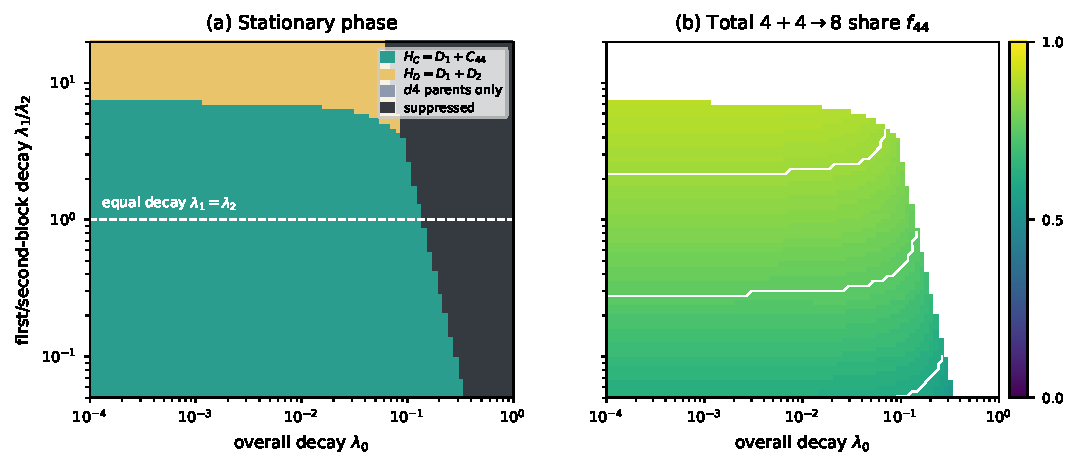
\includegraphics[width=0.96\textwidth]{fig_two_block_d4_d8_layerwise_phase.pdf}
\vspace{-7pt}
\caption{\textbf{Canonical $d4/d8$ stationary phase diagram.}  We set
$\gamma_4=\gamma_8=2$ and
$\lambda_E=\lambda_p=\lambda_8=\lambda_2=\lambda_0$, while varying
$\lambda_1/\lambda_2$.  (a) Global minima of Eq.~\eqref{eq:free8}.  The $H_C$ label means
that the block-2 route is $4+4\!\to\!8$; it does not require that this route carry all target
amplitude.  Large first-block decay shrinks the degree-4 representation until $D_2$ wins and
restores $H_D$, while large overall decay suppresses the tasks.  (b) Total compositional
share in $H_C$; white
contours mark $f_{44}=0.6,0.75,0.85$.}
\label{fig:phase8}
\end{figure}

\textbf{Interpretation and scope.}
The direct eight-singleton ReLU route is intrinsically inefficient, so the local threshold
$5/32$ is much easier to satisfy than the $1/\sqrt8$ threshold for $2+2\!\to\!4$.  This
explains the broad $H_C$ region in Fig.~\ref{fig:phase8}.  Nevertheless, high purity still
requires sufficiently large $\lambda_1/\lambda_2$, and this control eventually destroys the
parents' accessibility.  The main limitation is the omitted degree-2 leakage in
Eq.~\eqref{eq:relu4}.
Measuring those modes is essential in an experiment: if they feed the degree-8 output, the
observed circuit belongs to a larger multiroute theory rather than the two-family competition
derived here.

\begin{center}
\begin{tabular}{@{}lll@{}}
\toprule
Control & Desired movement & Limiting failure \\
\midrule
$\lambda_1\!\uparrow/\lambda_2$ & $f_{44}\uparrow$; suppress $D_1$ & degree-4 accessibility collapse \\
$\lambda_2\!\downarrow$ & move amplitude from $D_1$ to block 2 & larger block-2 norms \\
$\lambda_p\!\downarrow$ or $\gamma_4\!\uparrow$ & preserve degree-4 parents & weak parent regularization \\
$\lambda_8>0$ & fixes hidden/readout scale & degree-8 target suppression \\
$\lambda_E\!\downarrow$ & preserve singleton sources & embedding norms grow \\
project degree-2 leakage & isolate the two-family test & changes the architecture \\
\bottomrule
\end{tabular}
\end{center}

\end{document}
